\section{Current-Frame Incremental Validity}
\label{sec:primary_results}

\subsection{Primary Holdout Evaluation}
Table~\ref{tab:nested_models} presents the sealed holdout evaluation across nested model architectures on $N=255,164$ frames.

\begin{table*}[t]
\centering
\footnotesize
\setlength{\tabcolsep}{4pt}
\caption{\textbf{Primary Nested Model Evaluation on Sealed Holdout Cohort ($N=255,164$ frames, $2,804$ scenarios).} Models trained on all $15,641$ development scenarios and evaluated on the sealed holdout. Primary contrast is $M_{P+E_{\text{all}}}$ vs. $M_P$. Confidence intervals are pre-specified $95\%$ paired scenario-block percentile bootstrap intervals ($B=1,000$).}
\label{tab:nested_models}
\begin{tabularx}{\textwidth}{l l c c c c c c}
\toprule
\textbf{Model} & \textbf{Feature Set} & \textbf{Dim} & \textbf{AP} & \textbf{AUROC} & \textbf{Brier} & \textbf{$\Delta$AP vs. $M_P$} & \textbf{95\% CI} \\
\midrule
$M_P$ (Physical Baseline) & $P_{\text{clean}}$ & 12 & 0.3224 & 0.8022 & 0.0451 & Baseline & --- \\
$M_E$ (Context Only) & $E_{\text{all}}$ & 17 & 0.1141 & 0.7113 & 0.0516 & -0.2082 & [-0.2241, -0.1925] \\
$M_{P+E_{\text{static}}}$ & $P_{\text{clean}} + E_{\text{static}}$ & 17 & 0.3167 & 0.8046 & 0.0452 & -0.0056 & [-0.0157, +0.0038] \\
$M_{P+E_{\text{comp}}}$ & $P_{\text{clean}} + E_{\text{comp}}$ & 18 & 0.3157 & 0.8078 & 0.0453 & -0.0067 & [-0.0139, -0.0001] \\
$M_{P+E_{\text{interact}}}$ (Secondary Core) & $P_{\text{clean}} + E_{\text{interact}}$ & 18 & 0.3385 & 0.8347 & 0.0444 & +0.0161 & [+0.0057, +0.0264] \\
\textbf{$M_{P+E_{\text{all}}}$ (Primary Full)} & $P_{\text{clean}} + E_{\text{all}}$ & 29 & \textbf{0.3370} & \textbf{0.8399} & \textbf{0.0444} & \textbf{+0.0147} & [\textbf{+0.0005}, \textbf{+0.0285}] \\
\bottomrule
\end{tabularx}
\end{table*}

\begin{figure}[t]
\centering
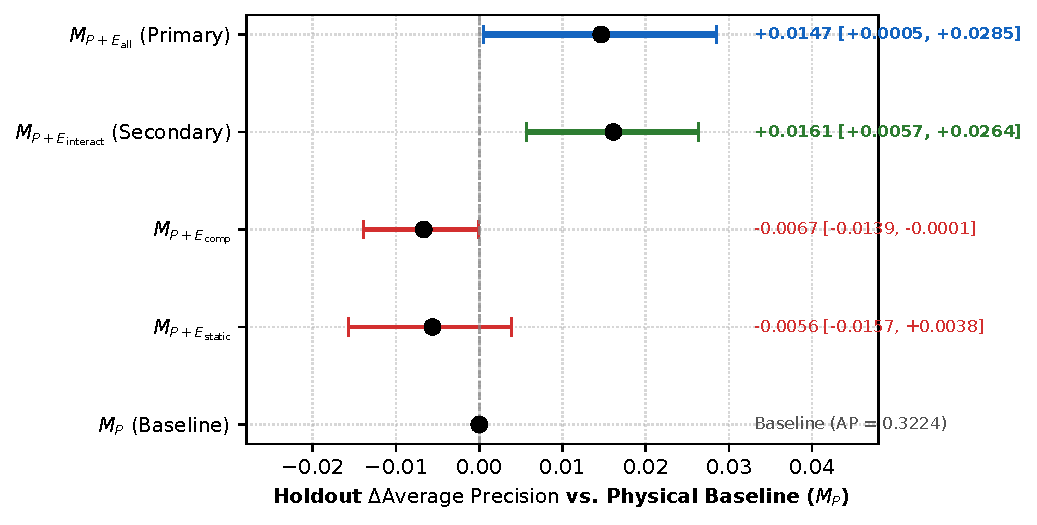
\includegraphics[width=\columnwidth]{figures/fig2_forest_plot_nested_models.pdf}
\caption{\textbf{Forest Plot of Holdout Model Contrasts.} Paired $\Delta\text{AP}$ and $95\%$ scenario-block bootstrap confidence intervals relative to physical baseline $M_P$. The full context model $M_{P+E_{\text{all}}}$ (primary) and interaction model $M_{P+E_{\text{interact}}}$ (secondary) achieve strictly positive lower bounds.}
\label{fig:forest_plot}
\end{figure}

The primary contrast supports a positive but modest conditional increment: AP increases from $0.3224$ to $0.3370$ ($\Delta\text{AP} = +0.0147$, $95\%$ CI $[+0.0005, +0.0285]$). The lower bound is close to zero, so the result should not be described as a large or practically universal improvement. The context-only model is substantially weaker than the focal baseline ($0.1141$ vs. $0.3224$), indicating that the proxies are useful conditionally rather than as a standalone replacement for focal kinematics.

\subsection{Individual Feature Replication}
Across the 13 pre-frozen candidate features evaluated in development, 10 out of 13 ($76.9\%$) achieved strict holdout confirmation with $95\%$ bootstrap confidence intervals strictly excluding zero in the expected direction. Furthermore, 13 out of 13 ($100\%$) demonstrated exact sign concordance between development and holdout splits, as illustrated in Figure~\ref{fig:feature_concordance}. Complete numerical breakdowns for all candidate features are provided in the Supplementary Material.

\begin{figure}[t]
\centering
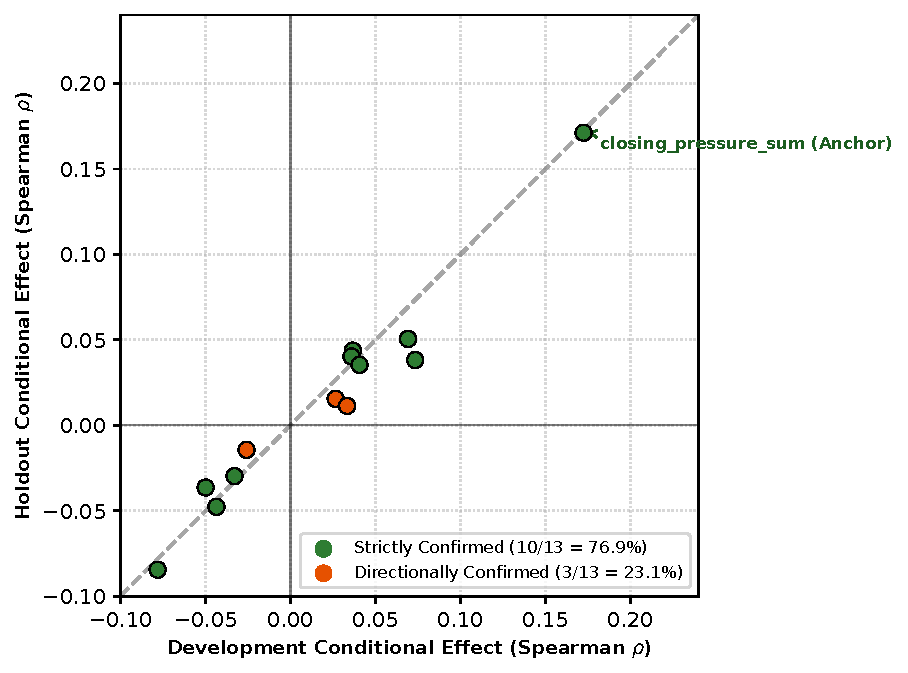
\includegraphics[width=\columnwidth]{figures/fig3_feature_concordance_dev_vs_holdout.pdf}
\caption{\textbf{Feature Effect Concordance (Development vs. Holdout).} Spearman rank correlation conditional effects across 13 candidate features showing $100\%$ sign concordance and $76.9\%$ strict confirmation.}
\label{fig:feature_concordance}
\end{figure}
